\section{Entorno de trabajo}
Para los cómputos de entrenamiento y predicción de la red se utilizó
una tarjeta gráfica (GPU, \textit{Graphics Processing
Unit}) \textit{Quadro K5000} de la marca
\textit{NVIDIA}\footnote{\url{https://www.nvidia.com/en-us/design-visualization/quadro-desktop-gpus/}}.
Tanto \textit{Deep-pose} como todas las herramientas utilizadas
para el procesamiento de datos fueron creadas con el lenguaje de
programación \textbf{Python} (versión 2.7) y con las bibliotecas
\textbf{Numpy} (versión 1.14.0)\footnote{\url{https://www.numpy.org/}}
para el manejo de los datos y \textbf{Theano} (versión
0.9.0)\footnote{\url{http://deeplearning.net/software/theano/}} para la creación
de la red.

\section{Entrenamiento de la red}
\textit{Deep-pose} se entrenó utilizando un algoritmo de
\textbf{descenso estocástico por el gradiente}
(SGD, \textit{Stochastic Gradient Descent}).
En este caso, SGD se utiliza para minimizar la función de costos sobre
un conjunto de entrenamiento $D$ que contiene poses tanto válidas como
señuelos. En cada iteración, un nuevo complejo $(x,y) \in D$ es
elegido al azar, donde $y=1$ si la pose es válida y $y=0$ en caso
contrario. Después la red, junto con los parámetros $\theta
= \{W^{b_{type}}, W^{b_{dist}}, W^{conv}, W^3, W^{out}, b^{conv},
b^{3}, b^{out}\}$ es utilizada para estimar la probabilidad
$p(y|x, \theta)$. Finalmente, el error en la predicción se computa
como la probabilidad logarítmica negativa, $-\log(p(y|x, \theta))$, y
los parámetros de $\theta$ son actualizados
utilizando retropropagación.
\begin{equation}
  \theta \longmapsto \sum_{(x,y) \in D} -\log p(y|x, \theta)
\end{equation}

En este trabajo, se utilizaron \textit{minilotes} de complejos, y
tomamos el promedio del error de la predicción para realizar la
retropropagación.

La red se entrenó con un conjunto de datos de \textbf{24,957 poses}
que se dividió en 19,965, 2,495 y 2,497 muestras para entrenamiento,
pruebas y validación respectivamente (80\%, 10\% y 10\%). Éstas poses al dividirlas
en ramas, resultaron en \textbf{5,216 distintas ramas}, que son las
utilizadas para crear el diccionario de ramas.

\begin{table}[H]
\begin{center}
\begin{tabular}{|c|c|c|}
\hline
Hiperparámetro & Descripción                         & Valor \\ \hline
\textit{N}     & Dimensión del vector característico & 80    \\
\textit{cf}    & Unidades en la capa convolucional   & 150   \\
\textit{h}     & Unidades en la capa oculta          & 60    \\
\textit{bs}    & \textit{Tamaño de los minilotes}    & 20    \\
$\lambda$         & Índice de aprendizaje               & 0.1   \\ \hline
\end{tabular}
\caption{Hiperparámetros utilizados para entrenar \textit{Deep-pose}.}
\label{tab:hyp}
\end{center}
\end{table}

El ajuste de los hiperparámetros se hizo de manera \textit{artesanal},
haciendo varias iteraciones de entrenamiento mientras se iban ajustando
los hiperparámetros. El mejor conjunto de hiperparámetros que se encontró
es el que se muestra en la tabla \ref{tab:hyp}.

\begin{figure}[H]
  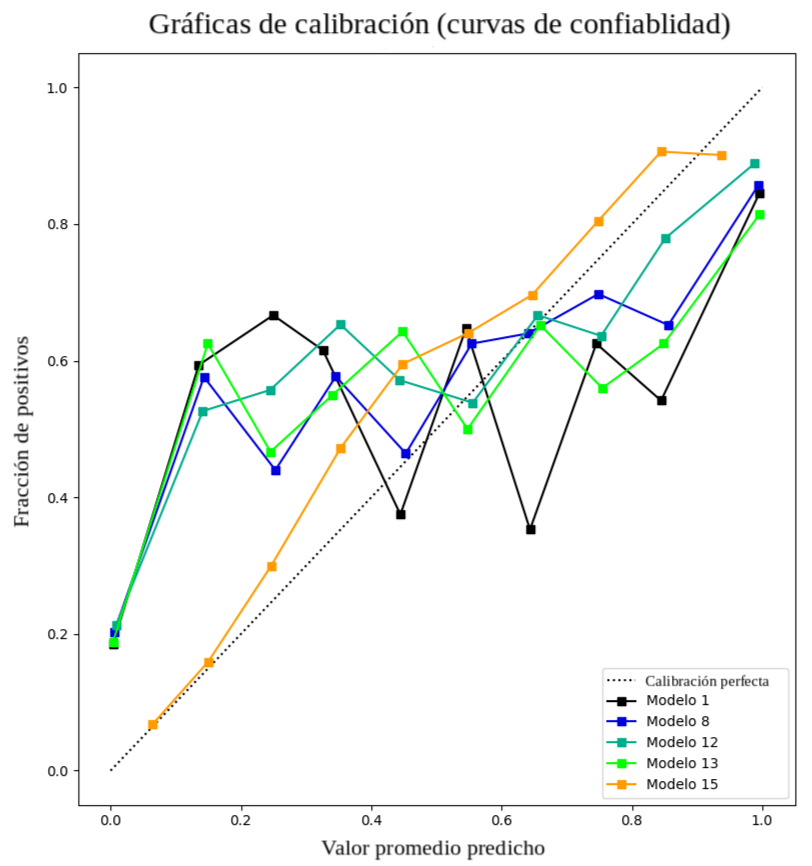
\includegraphics[scale=0.4]{calibration} \centering \caption{Calibracion
  de los hiperparámetros, siendo el modelo número 15 la mejor
  encontrada.}
\end{figure}

\section{Resultados}
Podemos ver en la figuras \ref{fig:confusion} y \ref{fig:roc}
que \textit{Deep-pose} alcanza una precisión de \textbf{82\%} al
momento de determinar si una pose es válida o no, lo cual muestra que
es una opción efectiva para determinar la fiabilidad de un
acoplamiento virtual.

\begin{figure}[h]
  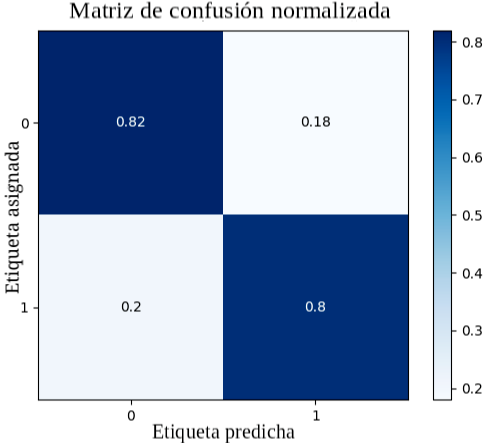
\includegraphics[scale=0.45]{confusion} \centering
  \caption{Matriz de confusión de las predicciones de la red,
  donde la etiqueta 1 representa una pose válida y 0 una inválida.
  Los puntajes son adquiridos a partir del conjunto de validación
  usado durante el entrenamiento.}
  \label{fig:confusion}
\end{figure}

\begin{figure}[h]
  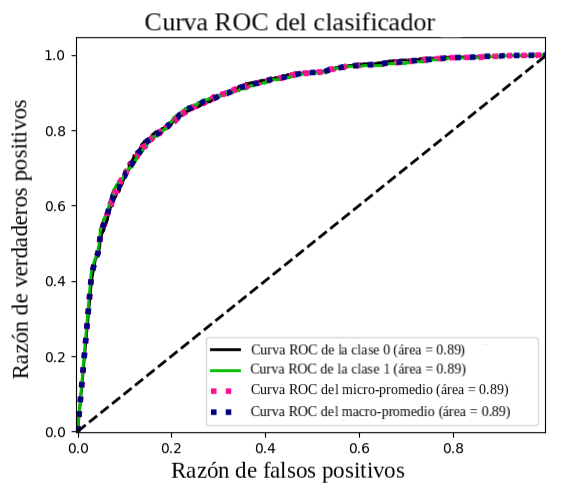
\includegraphics[scale=0.45]{roc_classifier} \centering
  \caption{Curva característica operativa del receptor (ROC,
  \textit{Receptive Operating Characteristic}) mostrando
  las razones de verdaderos y falsos positivos.}
  \label{fig:roc}
\end{figure}
